\documentclass[mathserif,serif]{beamer}
\usepackage{pdfpages} 
\usepackage{graphics}
\usepackage{amsmath,amssymb,amsfonts,textcomp,setspace,graphicx,lipsum,hanging,url}
\setbeamercolor{frametitle}{fg=black}
\begin{document}
  \begin{frame}
    \frametitle{\centerline{NFL Go For It!}}
    %Frame 1
In this project our goal is to help NFL coaches better determine when to attempt to go for a first down on a fourth down play.
  \end{frame}
  \begin{frame}
    \frametitle{\centerline{Slide 2}}
    %Frame 2
Explain the data you chose to answer these questions and why it is relevant.
  \end{frame}
\begin{frame}
 \frametitle{\centerline{The Research Question}}
In football there are many decisions a team needs to make in order win the game. In this project we focus on the decision that needs to be made on the 4th down of any given play. There are three decisions to be made on the fourth down. \\
\begin{enumerate}[1.]
\item 
Punt
\item
Kick a field goal
\item
Go for a first down
\end{enumerate}
In this project we try to determine which decision should be made under certain conditions. The following are the conditions which we take into account in determining the decision.
\begin{enumerate}[1.]
\item
Offensive and defensive rank of the offensive team.
\item
Offensive and defensive rank of the defensive team.
\item
The number of yards to convert a first down.
\item
The field position started from.
\end{enumerate}
With this information from the data we were able to estimate the expected points scored for each of the of three decisions.\\
Finally, with this information a decision can be made.
\end{frame}
  \begin{frame}
    \frametitle{\centerline{NFL Go For It!}}
    %Frame 3
\begin{figure}
\begin{center}
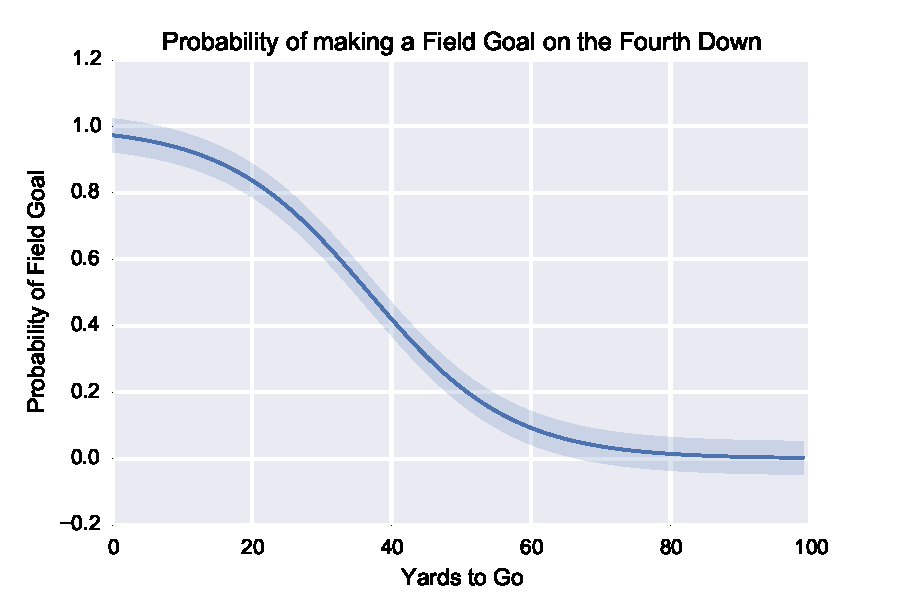
\includegraphics[width=1\textwidth]{fieldgoalprob.pdf}
\end{center}
\end{figure}
  \end{frame}
  \begin{frame}
    \frametitle{\centerline{NFL Go For It!}}
    %Frame 4
\begin{figure}
\begin{center}
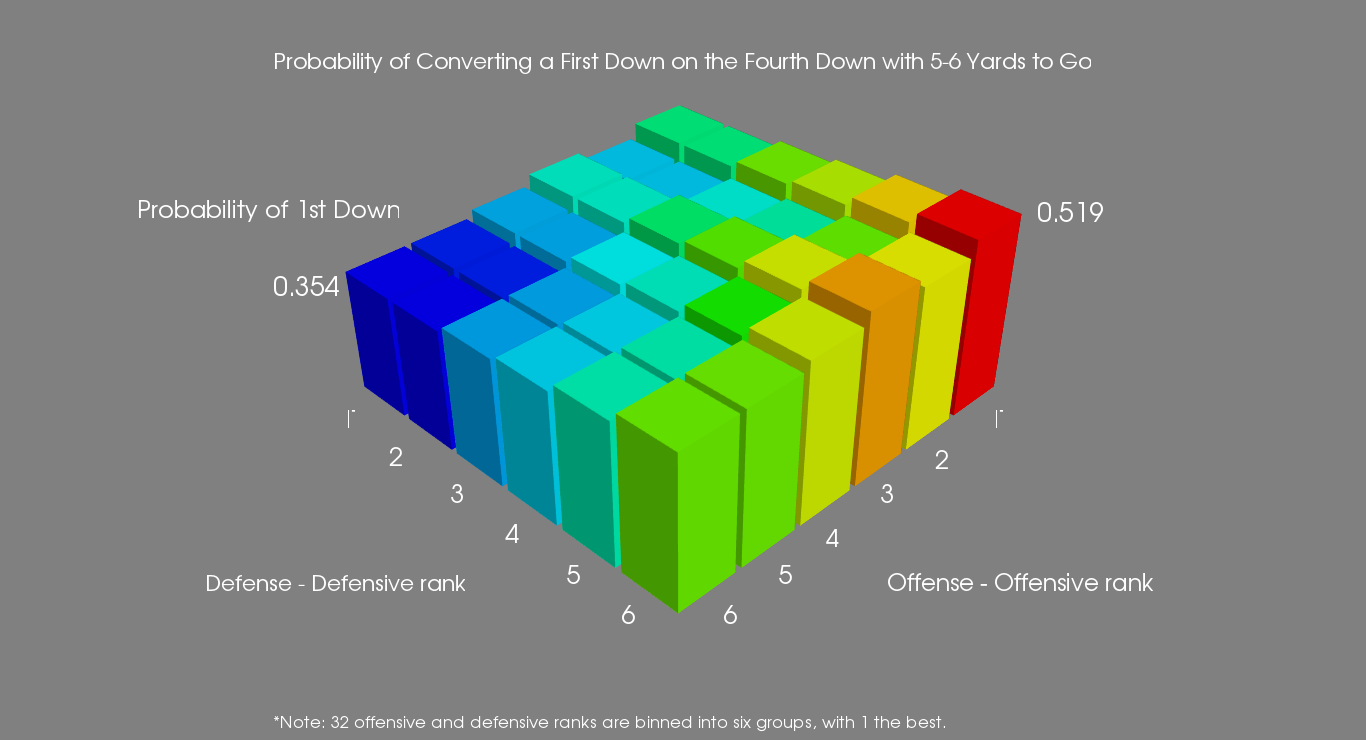
\includegraphics[width=1\textwidth]{ProbBarPlot.png}
\end{center}
\end{figure}
  \end{frame}
  \begin{frame}
    \frametitle{\centerline{NFL Go For It!}}
    %Frame 5
Show your answers to the questions, which are your final figures and/or tables. You should have the figure titles from your research proposal and now you should have the captions complete for every figure.
  \end{frame}
  \begin{frame}
    \frametitle{\centerline{NFL Go For It!}}
    %Frame 6
Show your answers to the questions, which are your final figures and/or tables. You should have the figure titles from your research proposal and now you should have the captions complete for every figure.
  \end{frame}
  \begin{frame}
    \frametitle{\centerline{NFL Go For It!}}
    %Frame 7
Show your answers to the questions, which are your final figures and/or tables. You should have the figure titles from your research proposal and now you should have the captions complete for every figure.
  \end{frame}
\end{document}